\documentclass[tikz,border=3pt]{standalone}
\usepackage[T1]{fontenc}
\usepackage{tgheros}
\usepackage{newtxmath}
\usetikzlibrary{arrows.meta,calc}
\renewcommand{\familydefault}{\sfdefault}
\definecolor{ink}{HTML}{20313E}
\definecolor{news}{HTML}{245E81}
\definecolor{risk}{HTML}{955230}
\definecolor{bluewash}{HTML}{EAF3F8}
\definecolor{claywash}{HTML}{FAF0E7}
\definecolor{muted}{HTML}{596C78}
\begin{document}
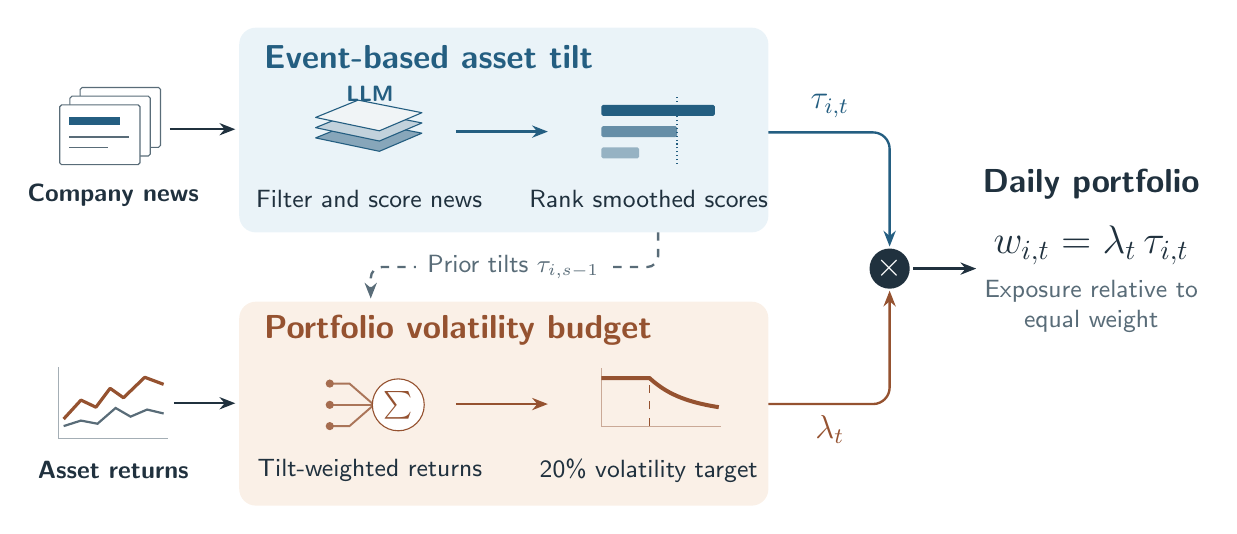
\begin{tikzpicture}[x=1cm,y=1cm,font=\sffamily\small,text=ink,
    arr/.style={-{Stealth[length=2mm,width=1.55mm]},line width=.85pt,draw=ink},
    module/.style={anchor=west,font=\bfseries\large,inner sep=0pt},
    oplabel/.style={font=\small,align=center,inner sep=0pt},
    source/.style={font=\bfseries\small,align=center,inner sep=0pt}]
% Modules own the broad surfaces; data and intermediate representations are glyphs.
\fill[bluewash,rounded corners=6pt] (2.62,3.42) rectangle (9.34,6.02);
\fill[claywash,rounded corners=6pt] (2.62,-.05) rectangle (9.34,2.54);
\node[module,text=news] at (2.93,5.65) {Event-based asset tilt};
\node[module,text=risk] at (2.93,2.18) {Portfolio volatility budget};

% Company documents and the input price panel.
\foreach \x/\y in {.60/4.50,.47/4.39,.34/4.28}{
  \draw[fill=white,draw=muted,rounded corners=.7pt] (\x,\y) rectangle +(1.02,.76);
  \fill[news] (\x+.12,\y+.51) rectangle +(.64,.09);
  \draw[muted,line width=.5pt] (\x+.12,\y+.35)--+(.76,0) (\x+.12,\y+.22)--+(.49,0);
}
\node[source] at (1.02,3.89) {Company news};
\draw[arr] (1.74,4.73)--(2.57,4.73);
\begin{scope}[shift={(.32,.80)}]
\draw[muted!55] (0,0)--(0,.91) (0,0)--(1.40,0);
\draw[risk,line width=1.15pt,line join=round] (.07,.25)--(.29,.49)--(.48,.40)--(.66,.64)--(.83,.52)--(1.1,.78)--(1.34,.69);
\draw[muted,line width=.8pt] (.07,.16)--(.29,.23)--(.50,.19)--(.73,.39)--(.92,.28)--(1.13,.37)--(1.34,.32);
\end{scope}
\node[source] at (1.02,.40) {Asset returns};
\draw[arr] (1.79,1.25)--(2.57,1.25);

% A language model and its filtered, ranked output.
\begin{scope}[shift={(4.28,4.62)}]
\foreach \h/\shade in {0/55,.13/28,.26/7}{
  \draw[draw=news,fill=news!\shade,line join=round]
    (-.69,\h)--(-.15,\h+.22)--(.66,\h+.06)--(.12,\h-.17)--cycle;}
\node[text=news,font=\bfseries\footnotesize,inner sep=0] at (0,.56) {LLM};
\end{scope}
\node[oplabel] at (4.27,3.84) {Filter and score news};
\draw[arr,draw=news] (5.37,4.70)--(6.54,4.70);
\begin{scope}[shift={(7.22,4.36)}]
\foreach \y/\w/\c in {.54/1.44/100,.27/.96/70,0/.48/48}{
  \fill[news!\c,rounded corners=.6pt] (0,\y) rectangle +(\w,.14);}
\draw[news,densely dotted] (.96,-.07)--(.96,.78);
\end{scope}
\node[oplabel] at (7.82,3.84) {Rank smoothed scores};

% An explicit one-period delay links relative allocation to risk estimation.
\draw[arr,draw=muted,dashed,rounded corners=4pt]
   (7.94,3.42)--(7.94,2.98)--(4.29,2.98)--(4.29,2.58);
\node[fill=white,inner xsep=4pt,inner ysep=1pt,text=muted,font=\small]
   at (6.10,2.98) {Prior tilts $\tau_{i,s-1}$};

% Weighted aggregation and the capped exposure rule.
\begin{scope}[shift={(3.77,1.23)}]
\foreach \dy in {-.27,0,.27}{
  \draw[risk!80,line width=.7pt] (0,\dy)--(.25,\dy)--(.56,0)--(.73,0);
  \fill[risk!85] (0,\dy) circle (.052);}
\node[circle,fill=white,draw=risk,text=risk,inner sep=1.5pt] at (.87,0) {$\sum$};
\end{scope}
\node[oplabel] at (4.28,.40) {Tilt-weighted returns};
\draw[arr,draw=risk] (5.37,1.24)--(6.54,1.24);
\begin{scope}[shift={(7.22,.96)}]
\draw[risk!50] (0,0)--(1.52,0) (0,0)--(0,.74);
\draw[risk,dashed,line width=.5pt] (.61,0)--(.61,.61);
\draw[risk,line width=1.45pt] (0,.61)--(.61,.61) .. controls (.82,.42) and (1.05,.31) .. (1.49,.24);
\end{scope}
\node[oplabel] at (7.82,.40) {20\% volatility target};

% Two current signals feed one portfolio decision.
\draw[arr,draw=news,rounded corners=6pt] (9.34,4.69)--(10.88,4.69)--(10.88,3.24);
\node[text=news,font=\large] at (10.12,5.02) {$\tau_{i,t}$};
\draw[arr,draw=risk,rounded corners=6pt] (9.34,1.24)--(10.88,1.24)--(10.88,2.68);
\node[text=risk,font=\large] at (10.12,.92) {$\lambda_t$};
\node[circle,fill=ink,text=white,minimum size=.51cm,inner sep=0pt,font=\large] at (10.88,2.96) {$\times$};
\draw[arr] (11.18,2.96)--(11.98,2.96);
\node[font=\bfseries\large,align=center] at (13.44,4.03) {Daily portfolio};
\node[font=\Large] at (13.44,3.25) {$w_{i,t}=\lambda_t\,\tau_{i,t}$};
\node[oplabel,text=muted] at (13.44,2.48) {Exposure relative to\\equal weight};
\end{tikzpicture}
\end{document}
